\subsection{Data Models}
The data used in the land use model system can be described as an integrated Data Model.
There are available graphical tools, including Visio, that facilitate the creation of Entity-
Relationship Diagrams to represent one view of a data model, such as the model presented in 
Figure \ref{figDataModel}.  This data model reflects in the upper portion essentially the data 
model used in SAM-IM (though we did not find any E-R diagrams in the documentation, and this 
diagram is based on interpretation of the documentation).

The key tables in the current SAM system are the exlu, plan, and developments attribute tables and
contents tables (which have a many to one relationship with the attribute tables to allow mixed use
representation).  There are no direct primary key - foreign key relationships that allow a database
join among these three attribute tables.  Instead, they are spatially cross-referenced by the 
conversion to grids.  The various geographies used in SAM and their relationships are included
in the top part of the E-R diagram, including census blocks, block groups, tracts, taz, raz, mpa,
county, and state geographies.

The bottom part of the diagram augments this data model by showing the possible entities and their
relationships is a fully detailed data representation is adopted for this project, either in the
short run (phase 1) or later.  This portion of the diagram shows the key entities of persons, 
households, jobs, businesses, buildings, and parcels.  The model could be simplified by eliminating
persons, or businesses, for example, or collapsing buildings into parcels, or by aggregating 
parcels into larger land use polygons (potentially into development sites).  Any aggregation involves compromises, however, and these compromises should be considered carefully.  Our proposal at this point is to use the most disaggregate representation possible given the available data, which may vary across different parts of the region.  In this case, different data models would be developed to represent the
starting condition in each area, and a data model representing the target database would be developed
as well.


\begin{figure}[h]
\begin{center}
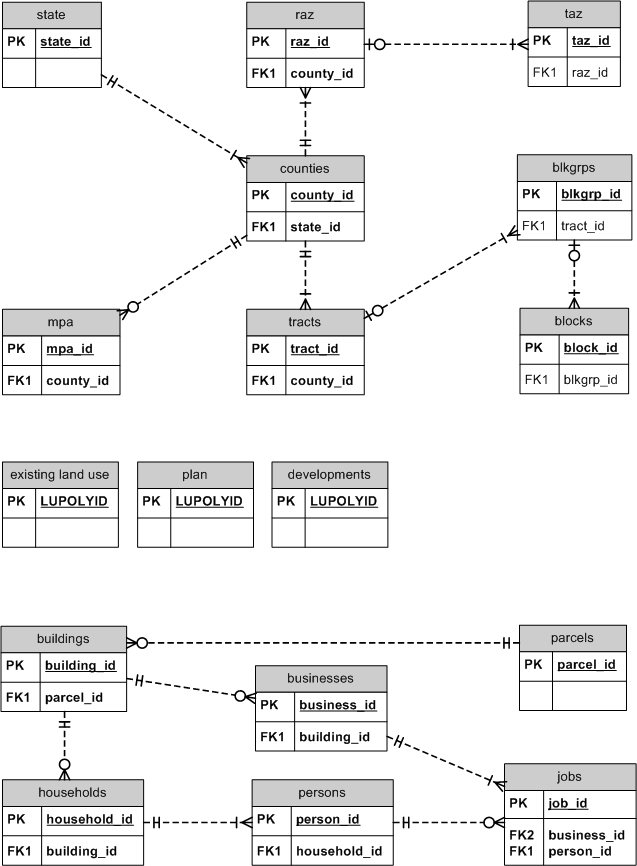
\includegraphics[scale=0.5]{figures/AZ-SMART_data_model_diagram.png}
\caption{AZ-SMART Data Model}
\label{figDataModel}
\end{center}
\end{figure}